%\chapter{Compact Object in Globular Clusters}
\chapter{Introduction}
\thispagestyle{fancy}

\section{Location, Location, Location}

Important in real estate, but also seems to be an important factor to take into account when studying compact objects in binary systems. It seems that, like with people, where you were born plays a role on your formation and evolution. This seems to be true for cataclysmic variables (CVs), the kind of compact binary system that we will explore in more detail in the present work. Our goal is to try to understand the formation of these kind of systems when they are formed in a crowded and high density environment (like in a cluster of stars), and when you give them enough time to evolve and interact with other stars (like in a globular cluster). \\ 

Now that we have defined our broad goal let's take a step back and explore in more details what are compact objects, their different types, and the different ways they can interact with each other and other types of stars (Sec. \ref{sec:co}). That section will lead us to the discussion of where and how we expect to find them, and what can we learn by studying them in the different environment where they form (sections \ref{sec:gc} and \ref{sec:spec}).

\section{Compact Objects or Stellar remnants}\label{sec:co}

Compact object, as their name suggest, are very massive and dense objects formed from the remains of a dying stars; hence their other name stellar remnants. They come in three different flavors, each following a different formation mechanism that is mainly determined by the mass of the progenitor star (do I need a reference for this?). The different types are neutron stars, black holes, and white dwarfs. Besides these three, other possible exotic types of stars have been proposed. Including quark stars, boson stars, and Thorne-Zytkow objects. These will not be discussed in this work as there is still lack of physical observational evidence on there existence. The reader is refer to the following references if so inclined to know more about these particular kind of proposed stars. (Find references for exotic stars). \\

%Let's begin our discussion with the neutron stars, the densest type of stars hitherto observed.

%\subsection{Neutron Stars: Nature's lighthouses}\label{sec:ns}
\subsection{Neutron Stars}\label{sec:ns}

Neutron stars, first proposed in 1934 by Baade and Zwicky,  are stars where the sustaining force against gravity comes from  the degeneracy pressure between neutrons \citep{baade_cosmic_1934}. These stars are produced from the gravitational collapse of a massive star (> 8 M$_\odot$)(ref for mass range) at the end of its life. The supernova produced by this collapse, lefts behind a dense and massive core. A core of a couple of kilometers in radius (exact number?), but sustaining possible up to $\sim 2$ Solar mas (ref for max observed NS or Oppenhiemr limit). They are mainly  composed of neutrons and a thin atmosphere of a few cm of Hydrogen and other heavier elements (ref for NS atmosphere models). We have come a long way since the first proposition of their existence, but there still a lot of  uncertainty on their interiors and a lot of existing conflicting models. Since we have had observational evidence on their existence (ref first observational evidence, maybe first pulsar PSR B1919+21?) efforts have been done to constraint the different physical models. Figure~\ref{fig:nsmod} shows a visual summary of the different models proposed. There are many ways that we can observationally constraint these models, spectroscopy being one of them. Spectroscopy is still the gold standard for observational astronomy of the electromagnetic spectrum. The advantages of using spectroscopy to study compact objects is discussed later in section~\ref{sec:spec}. The focus of that section is on the advantages of spectroscopy for the study of white dwarfs, but the same applies to systems with a neutron star object. The details on the future plans on how to use MUSE data to constraint such models of a neutron stars are left for the future work section (\ref{sec:futur}).


It is important to note that these dense objects are expected to be formed as isolated objects, but are also known to be found in binary system. They can interact with other compact objects and main sequence (MS) stars~\footnote{Main sequence stars are those that for millions of years spend their time burning hydrogen at their cores.}. The impatience reader can skip to sec~\ref{sec:cb} for more details on the kind of binary systems in which we expect to find a neutron star. We now continue with our discussion of other types of compact object. The next in line being probably the one who gets more attention out of all the compact objects: black holes.


\begin{figure}[]
        \centering
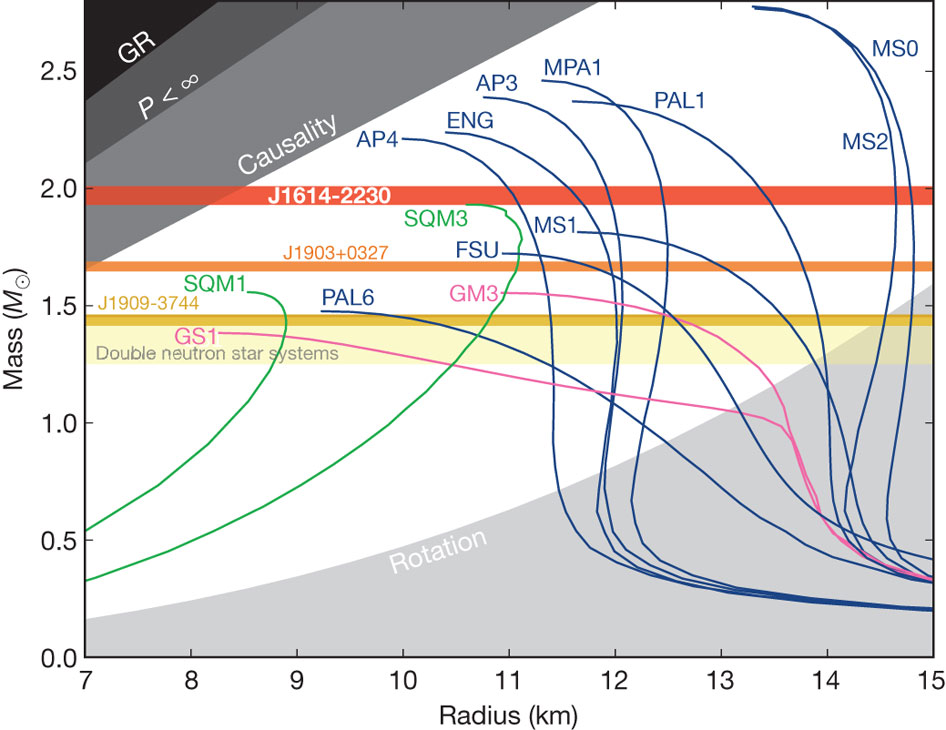
\includegraphics[scale=.3]{assets/images/es.jpg}
\caption{The plot shows non-rotating mass versus physical radius for several typical equation of states.  Blue, nucleons; pink, nucleons plus exotic matter; green, strange quark matter from (doi:10.1038/nature09466)}
\label{fig:nsmod}
\end{figure}


\subsection{Black Holes}\label{sec:bh}

The term was coined by John Wheeler in 1968 (reference for the term), but the idea about an object so massive that don't even light could escape have been around for centuries (Ref. for Laplace 1700s). Like neutron stars they are the fate of really massive stars. In this case even more massive objects were no known force can fight gravitational attraction. 

These are fascinating objects and a lot can be said about them. They have been extensively studied and indirectly observed across the electromagnetic spectrum, and most recently with gravitational waves observatories (LIGO ref \cite{a}). But we won't discussed them anymore in here. They will be briefly mentioned again when discussing the population of compact objects expected to be found in the dense regions of our galaxy halo (globular clusters~sec~\ref{sec:cogc}). 

Now we pass to the last type of known compact object: white dwarfs. They will be the subject of most of the rest of this report. 

\subsection[White Dwarfs]{White Dwarfs: The poor star's fate}\label{sec:wd} 

White dwarfs are by far the most common type of compact objects. It is the fate of most main sequence stars when they burn all the available hydrogen in their cores (give percentage and citation \cite{a}). This will also be the ending of our own Sun several billions years from now. Something so common, yet so unknown. It is true that thanks to the development of quantum mechanics and multi-wavelength observation of these objects (gravitational waves observation of these objects will have to wait until the eLISA mission (ref. to eLISA\cite{a})) we have learned a great deal about them, but still a lot of uncertainty surrounds them. Specially on their formation and evolution when in a binary system. That is the main motivation behind this work. But now lets take a step back and defined precisely what are white dwarfs and briefly discussed what we do know about them. 

White dwarfs, like neutron stars, are supported by the degeneracy pressure. In the case of a white dwarfs this pressure is due to the electrons and not the neutrons. But unlike neutron stars the progenitor star (a MS star of > 8 M$_\odot$ \cite{a} Ref. Needed) has a more complex history leading to the formation of the compact object. A qualitatively picture of the evolution of the progenitor star as it "moves" around the Hertzsprung-Russell (HR) diagram\footnote{ The Hertzsprung-Russell or HR diagram is basically a log-log plot of luminosity $L$ vs. effective temperature. This is widely use in astronomy.} is shown in figure~\ref{fig:hrwd}. The field of stellar evolution is an active and complex area of research and the reader is invited to read \cite{koester_physics_1990} for a more detail review of the physics and evolution of white dwarfs. For now the details of the evolution of the progenitor star of the white dwarf is not so important, but it is a good way to introduce the HR diagram. The HR diagram is an useful tool and the names of the different regions indicated in the HR diagram presented in figure~\ref{fig:hrwd} is something to bear in mind for the rest of this report.  

\begin{figure}[]
        \centering
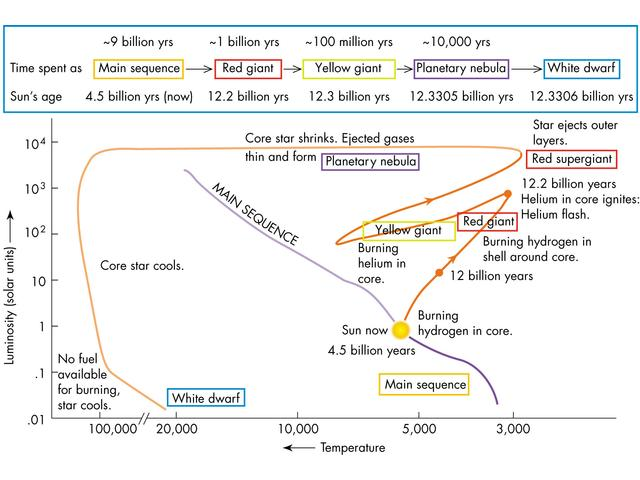
\includegraphics[scale=2]{assets/images/starevol.jpg}
\caption{Evolution Sun-like star to white dwarf. Source: The sloan digital sky server data \protect\url{http://skyserver.sdss.org/dr1/en/astro/stars/stars.asp}}
\label{fig:hrwd}
\end{figure}

Continuing our comparison between the different compact objects, it only left to say that white dwarfs are too expected to be found in binary systems. These binary systems formed from a compact object are the topic of the next section. 


\begin{comment}
very energetic events that result from i

Exotic interacting binaries with collapsed stars are among the most powerful energy sources in the Universe, outshining their host galaxies. Interacting binaries are a rich laboratory for a wide variety of astrophysical phenomena.
Mention violente mechanism as novae anddwarf novae. Study the nature of accretion. An universal phenomena present at many scales. 
\end{comment}


\section[Compact Binaries]{Compact Binaries: Nature's "Death Stars"}\label{sec:cb}

Here we will explore a small part of the vast compact binary zoo. In doing so we will be studying some of the most powerful events in the universe. These powerful events are the result of the interactions between a massive and extended object (main sequence star e.g. our Sun), an even more massive and dense object (neutron star or white dwarf).  These interactions can result in flashes of light capable of competing in brightness with their host galaxy. In fact, these objects have only been discovered relatively recently when humans have been able to observed the sky in high energy electromagnetic radiation, X-Rays. The first discrete X-Ray source in the universe was discovered in 1962 by Giacconi et al, named Sco X-1. The results were published in a landmark paper titled "Evidence for X-Rays from sources outside the solar system". These sources are now known to be several orders of magnitudes brighter in X-Ray than our Sun ($\sim 1 \times 10^{38} \text{ ergs s}^{-1}$~\citep{firstxray} vs $\sim 1 \times 10^{28} \text{ ergs s}^{-1}$ \citep{sunxray}). This first X-ray source, Sco X-1, have been widely studied for more than 50 year in all wavelengths and it represents the prototype low-mass X-ray binary (LMXB). So let's talk next about what is a LMXB and how they are related to compact objects.  

%Let's begin by revisiting the neutron star and see how this powerful X-Ray emission can be produced from the gravitational energy of a binary system.  

\subsection{Low-Mass X-Ray Binary}

A low-mass X-ray binary is composed of a neutron star and a low-mass late-type star (sometimes refer as the secondary or companion star). What is important in this scenario is that the companion star fills what is called the Roche lobe. The Roche lobe represents the area of influence of a star in a binary system. Inside the Roche lobe of an object the material will be gravitationally bound to that object. If the secondary star fills its Roche lobe, material can be transfer to the compact object (in the case of a LMXB a neutron star). This mass transfer is called "Accretion". If the accreting material have some initial angular momentum it cannot fall radially into the more compact object but it will slowly fall into the compact object and form what it is called an "accretion disk". An sketch on how this happens can be seen in Fig~\ref{fig:lmxb1}.

The specific accretion scenario described above was first proposed by \cite{acre68}. This was not the first model to explain the X-ray emissions from these object. The first attends were done by \cite{shklovskii_nature_1967} and even before by \cite{hayakawa64}. The models all proposed high-temperature infalling gas into a very massive and dense object. But \cite{acre68} model takes into account the angular momentum of the infalling plasma, and thus the formation of a disk. Concluding that "the optical radiation will be emitted from the outer parts of the disk and the X-Rays from the inner part." \citep{acre68}. The model was developed for accretion in a white dwarfs but it also extents to neutron stars. The first accretion disk model for neutron star accretors came in \citeyear{pringle_accretion_1972} from \citeauthor{pringle_accretion_1972}. This model mentioned the fact that around the neutron star the magnetic field controls the gas dynamics. This would mean that the X-Ray emmisions also come from the regions on the stellar regions near the poles. 

Here we only touch the basics on the accretion phenomena that are present in some compact binary systems. A more detail look into the physics can be found in \cite{pringle_accretion_1981} and a more recent book is \cite{frank_accretion_2002}. We will revisit the subject of accretion disks in sec.~\ref{sec:spec} when we see why we need spectroscopy to better understand the nature of the compact binaries and their accretion disks. 

Now that we have seen in what kind of binary system neutron stars can be found, we can turn the page and study white dwarfs in binary systems.   

%is what produces the powerful X-Ray emissions that led to their discovery. The transfer material from the secondary star heats up as it falls to the compact object losing gravitational potential energy. 

%Conversion of gravitational potential energy to radiation. 
%to the emission of the X-Ray that   
%The accretion disk is an important component of a compact binaries.  %As it was said in the last section, LMXB are powerful emitters of X-Rays. 

\begin{figure}[]
        \centering
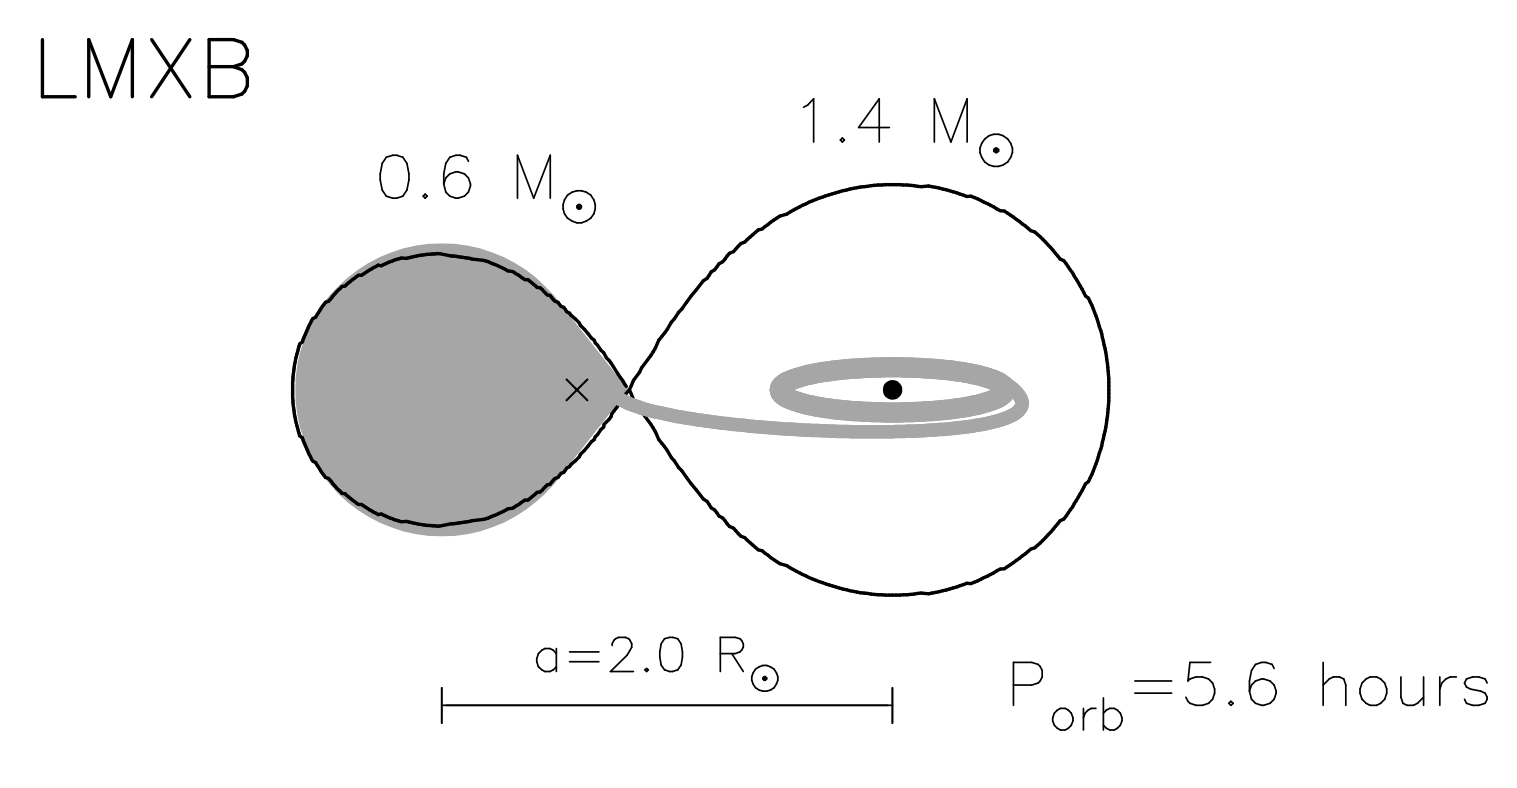
\includegraphics[scale=.3]{assets/images/lmxb1.png}
\caption{The plot shows a cartoon representation of a LMXB from \cite{lmxb1}. The black lines represents the Roche lobe. In this picture the companion star fills its Roche lobe and so material is transfer into the neutron star. The material from the star forms what is called an accretion disk due to the initial angular momentum of the accreting material from the star. }
\label{fig:lmxb1}
\end{figure}

\subsection{Cataclysmic Variables}

Like with the neutron star we start by examining what happens when a compact object (in this case a white dwarf) accreates from a main sequence star due Roche lobe overflow. In this case the name is not as descriptive as for the LMXBs, they are called Cataclysmic Variables (CVs). They, like LMXB, are sources of X-Ray and optical radiation coming mainly from the accretion disk surrounding the white dwarf. 

CVs might be formed from the most common compact object (white dwarfs), but by no means this lower their ranking in the compact binaries group. Like LMXB they have been studied since the dawn of X-ray astronomy, and even further back with optical observation. In fact the first discussion of accreation in a CV goes back to the year \citeyear{crawford_intrepretation_1956} by \citeauthor{crawford_intrepretation_1956}. In the paper \citeauthor{crawford_intrepretation_1956} proposed a model for AE Aqr that involved gas transfer from the primary to the white dwarf. This was done a mere 18 years after the discovery of AE Aqr as a rapid variable star in \citeyear{zinner_mitteilungen_1938} by \citeauthor{zinner_mitteilungen_1938}.  

These are fascinating objects with a rich range of behaviours, including really energetic outburst that give rise to the name cataclysmic variables. They are the main subject of study of this work, but before we can say anything more about them we need to explore the vast taxonomy of these objects. %We begin by looking at the classification of CVs.  

\subsubsection{Magnetic CVs}

Easy enough these are CVs for which the magnetic field is strong. The actual definition is a bit more complex involving synchronization of orbit and rotation, and modulation of X-rays; but we don't need to know the details now. The main idea is that in the presence of a strong magnetic field the accretion flow can be disrupted. This disruption can be partial or complete. This then gives rise to a subdivision of these objects: Polars and Intermediate Polars.  They both share some characteristics. In both type of systems seem to be very variables (other of magnitudes and ref for this). They also share some spectral properties, the most noticeable one being the presence of Helium II. This is due to the ionized accreting plasma. 


\subsubsection{Polars}

Polars are a type of CV where the magnetic field is strong enough to control de flow of the material near the white dwarf. The term was first coined by \cite{krzeminski_extremely_1977} due to the high degree of polarization (both circular and linear) found in these type of systems. The polarization was the first clue on the magnetic nature of these type of systems. It was first discovered for AM Herculis (AM Her), now the prototype polar CV (\cite{tapia_discovery_1977}). In fact Polar systems are somethings referred as AM Her-like system. 

%AM Her was first discovered in \citeyear{ref} by \citeauthor{ref}. Later study of the spectra and of the X-ray emissions show strong v(\cite{ref} Ref for AM HER).  

%Locked orbit ot synchonyze rotation

\subsubsection{Intermediate Polars (IPs)}

The second kind of magnetic CVs are those where the magnetic field is not negligible but also it is not strong enough to completely dominate the accretion flow. They are called Intermediate Polars. The first two classified members are TV Col and AP Psc. They showed AM Her-like spectra, but no sign of strong polarization (Ref. needed \cite{ref}). Another very well know member of this class is DQ Her. DQ Her is somethings refer as a subclass of IPs, or even as a synonym for IP. A 30 pages review, a bit outdated, dedicated solely to the topic of DQ Her stars and IPs is \cite{patterson_dq_1994}.  


\subsubsection{Non-Magnetic}

As opposed to the magnetic CVs, the magnetism doesn't interfere significantly with the accretion from the secondary stars. These doesn't mean that these CVs are "well-behaved" and less variable than the magnetic ones. Au contraire, these kind of CVs are known to display an eruptive behaviour. In fact, they were the first kind of CVs to be detected and the reason they carry the infamous name, cataclysmic variables. Non-magnetic CVs (for the most part. Some exceptions are known e.g. \cite{a} I think DQ Her but have to check and  V1500 Cyg from Pagnotta et al 20016) are the source of very powerful outbursts. There are the two kind of eruptions observed in CVs and they define the different types of non-magnetic CVs. %The types are classical novae, dwarf novae, nova-like and recurrent novae. 


\subsubsection{Classical Novae (CN)}

When the surface of an accreting white dwarf becomes hot enough, nuclear fusion can take place and a thermonuclear runaway happens. This creates a violent explosion capable of ejecting material at high velocities. These outburst are fairly easy to detect since they cause a substantial increase in brightness (6-19 magnitudes \cite{a} Find reference). A CV observed erupting in such a way is classified as a \emph{classical novae}. By definition a CN have been seen to erupt only one. If a previously recognized CN erupts again as a CN they are called recurrent novae. 

Classical novae are the most violent non-destructive eruption observed from a CV, but not the only one. Another kind of instability can cause violent outburst in a CV and gives the name to the second type of non-magnetic CVs, dwarf novae. 


\subsubsection{Dwarf Novae (DN)}

An dwarf novae outburst in an eruption caused by instabilities in the accretion disk. This is predicted to happened in non-magnetic CVs with low accretion rates. They usually not happen in magnetic CVs because as stated in \cite{shara_erupting_2005}: "Magnetic fields in CVs are usually expected to prevent the disk instability that leads to dwarf nova eruptions". There are some few exceptions like EX Hya (ref for this \cite{a}). CVs that show dwarf novae outburst are classified as dwarf nova. The outburst from a dwarf nova is not as violent as the one from a classical novae. The magnitude change is only of about 2-5 (\cite{ref} get ref for this), and no material is ejected. They also, unlike classical novae, are periodic in nature with a well defined time scale depending mainly on the accretion rate.  

For the details on the nuclear physics governing DN see\cite{shara_recent_1989} and a very recent one from \citeyear{starrfield_thermonuclear_2016} by \citeauthor{starrfield_thermonuclear_2016}. \\



\subsubsection{Novae-like (NL)}

Another classification of white dwarfs that I haven't mentioned is the novale-like one. These are a bit ambiguous as both magnetic or non-magnetic systems can be classified as NLs. They are basically CVs that seem to have stable accretion, thus not undergoing dwarf novae outburst and having a bright stable disk. So even if you would guess from the name, this represent the 'non-eruptive' CVs. \\

A lot of new terms have been defined here I apologize for that, but this also shows how rich variety of behaviours present in CVs. So far we have focused our discussion of CVs based on the nature of only the white dwarf, after all these are the main driver of systems. But before we can pass to another topic we have to discuss a bit the nature of the secondary stars in CVs. 


\subsubsection{The Secondary stars}


The detailed study of the secondary stars in CVs can be on its own the sole topic of a thesis. Here we limit the discussion for late-type stars.  This is justified by the fact that we will be studying CVs in globular clusters. Globular clusters, as we will see in the next section, are very old clusters of stars, so the most common stars in the cluster are expected to have relatively small mass (Do i need to cite this). In fact for NGC 6397, the globular cluster studied in this work, the turnoff mass~\footnote{the turn off mass is the maximum mass on the main sequence. This can serve as a rough estimate of the maximum mass of main sequence stars in a globular clusters.} is $0.77 M_\odot$ \citep{de_marco_spectroscopic_2005}. 

Late-type stars can be a term a bit ambiguous, but in this report the term will exclusively refer to K and M type stars. Let's look at them in more detail.  

\subsubsection{K stars}

Search for good reference for info. They are discussed in Natalie's thesis. Include specta?


\subsubsection{M stars}

Search for good reference for info. Include specta? \\



With the discussion of the secondary stars we end our discussion on compact objects and binaries. In this section we learned what compact objects are and explored two specific types of accreting binaries, LMXB and CVs. We briefly mentioned the characteristics of an LMXB, and then focused on the CVs. We studied the rich nomenclature of CVs, and the different types of CVs based on their outburst and magnetic properties. But I must say that I have only touch the surface of this ample topic. The following references are valuable sources for the avid reader that wish to know more about the subject. The first good source of information is Warner's book \emph{Cataclysmic Variable Stars} \citep{warner_cataclysmic_2003}, an essential reference for this topic. Another good reference at a lower level and easier to read is \cite{hellier_cataclysmic_2001}. 

A review that deals with the evolution of LMXB and CVs (the two only binaries mentioned here) is \cite{patterson_evolution_1984}. Another one that don't limit the discussion to white dwarfs and neutron star is the book \cite{frank_accretion_2002}. The book extends the discussion to all the compact objects (including black holes) and discussed the physics of the different models of accretion besides Roche overflow. \\ 

Now that we have a better idea about compacts objects, specially about CVs, the next sections will be about where can search for compact binaries, and how. \\ 

\begin{comment}
Meyer & Meyer-Hofmeister (1981, 1982, 1983) firstly discussed the physical mechanism responsible
for dwarf nova outbursts which is connected with the thermal instability of the disc which occurs in the
temperature range corresponding to the ionization of hydrogen. Soon after Smak (1984a,b) extended the
study of such a mechanism. The details are summarized by Smak (2002) as follows.
From 2008ChJAS...8..237G   Cataclysmic Variables: A Review Giovannelli

Dwarf novae belong to the class of nonmagnetic cataclysmic
variables in which the magnetic field of the white dwarf is too
weak to disrupt the accretion disk, so that the disk can extend
close to the surface of the white dwarf 

%(see Warner 1995 for a review of dwarf novae).
\end{comment}




\section{Globular Clusters: A stellar nursing home}\label{sec:gc}

%As we saw. We expect them to form in high density envrioment. Revew 
%
%Know distance for example. 

\subsection{NGC 6397}



\subsection{CVs in Globular clusters}\label{sec:cogc}


There are three open questions in this field:

\begin{enumerate}
        \item \textbf{Are all CVs in globlular clusters magnetic}
        \item \textbf{Where are all the primordial CVs?}
        \item \textbf{What are the periods of these white dwarfs}
        \item \textbf{Where are all the dwarf and novae?}
\end{enumerate}


\begin{comment}

As usnsual we will igonre BHs. I can briefly mentioned that they are expected to be found in GC. Briefly mentioned search for spectect Intermediate BH (reference), but concentreat on CVs
For a big reviw see (big reference of GC natalie old), and relativisitc binaries is worth looking (reference mathew benacquista). A great review on CVs is kigee CVs in GC. 


I hope I have convince you by now that compact objects are a class of objecsts worth studying. There mass and densities lets us prove into physics that is still not possible with modern technology. The violent phenomena happind at the different scales is an open laboratory for high energy physics and their exoctic and excentric cores still presents a challenge for nuclear physicist. 

I also hope that I made the point that cataclysmic variables are of special interest, as they represent the fate of our own star and possibly of the vast majority of stars. These are objects that are predicted to be so common, and yet far to be completely understood. 

It should also be clear by now after the discussion on globular clusters in the last section why we would expect and search for CVs in them. But what I haven't discussed is what is our current understanding on the issue. What have we learned in years of observation and more importantly what is still to learn about them. In other words what is the motivation



Natasha paper


There are three open questions in this field:

\begin{enumerate}
        \item \textbf{Are all CVs in globlular clusters magnetic}
        \item \textbf{Where are all the primordial CVs?}
        \item \textbf{What are the periods of these white dwarfs}
        \item \textbf{Where are all the dwarf and novae?}
\end{enumerate}

\textbf{Magnetism}

The look for He II. (Emmision lines) and line ratios. 

\textbf{Primordial CVs}

Balmer series

Bright vs faint H$\alpha$, period ? (We

What hasn't been discussed is what is the current undesrtading on the topics. 
We can expect to see emmision on absoption maybe


\textbf{Period gap: Is it real?}

We need more data and sp. Emission lines can help. 


\textbf{Where are all the dwarf and novae?}

These two are violent explotion


Optical spectroscopy is the answer
\end{comment}

\section{Spectroscopy: The golden standard}\label{sec:spec}

%"Photometry is not enough" could have been the name of this subsection. As discussed above specific emmision and absro 
%It is pretty clearn what data we need
  
The advances in spectroscopy have been tied with our understanding of compact binaries. This was recognized as early as \citeyear{zeldovich_collapsed_1966} by \citeauthor{zeldovich_collapsed_1966}. In this letter they wanted to "draw attention" to the study of "collapsed stars"and call to the find X-Rays from single-line spectroscopic binaries as "unambiguous proof of the existence of a collapsed star". For CVs this have also been the case. For example the idea that lead to the correct interpretation of accretion as an important agent in the variable systems like AE Aquarii only was possible after the its classification as a spectroscopic binary~\footnote{A spectroscopic binary is a binary where we see the periodic doppler shift of a line due to the orbit of the object.} \citep{joy_spectroscopic_1954}. Also spectroscopy have been an amazing tool used to prove and confirmed the presence of accretion disk in compact binaries. This is because emission lines bring key information about binaries, and specially about accreting binaries. They provide kinematic signature of accretion phenomena, and allow for the tracing of the accretion flow. This accretion disk is the dominating light at optical wavelength. The emitted lines from the accretion are highly structured and even time-dependent, in some cases. The most prominent features being the so called Balmer series (Hydrogen emission lines) and Helium lines (Helium I and Helium II). The Balmer lines from an accretion disk in a CV have been first studied by \cite{williams_emission_1980}. The expected characteristic double-peak hydrogen emissions were model already in the \citeyear{smak_emission_1981} by \citeauthor{smak_emission_1981} and expanded by \cite{horne_emission_1986}. Spectroscopy have also been a valuable tool to explore the physical properties of the compact objects, and not only of the accretion flow. For example presence of He II have been suggested to indicate "accretion 'curtains' along the magnetic field lines of the WD." \citep{edmonds_cataclysmic_1999}.  


%Mangetism in Helium Ii lines is a for magnetism (reference for this ). 
%
%.   as mentioned above. eIn white dwarfs for example we can look for the Helium emission lines, both He I and He II, to get more information about the magnetism and temperature of the accretion disk. He II is a sign of magnetism and He I can only be found in neutral accreting matter (ref for magnetism and accretion). And only spectroscopy can help with the correct classification of CVs in their different classes.  


In recent times with the advent of space exploration and construction of bigger telescopes. High resolution slit spectroscopy (both from space and from the ground) have allow us to improve our knowledge of the compact binaries. We pay special attention to the advancement in the study of CVs in globular clusters. The first of such studies was for the globular cluster M5 by \cite{margon_m5_1981}. Then 18 years after only three studies followed in two other globular clusters (\cite{deutsch_serendipitous_1999, grindlay_spectroscopic_1995,edmonds_cataclysmic_1999}).  

After 1999 the next spectroscopic study of compact objects in globular clusters had to wait until de development of the technique called \emph{slitless spectroscopy}. This was proposed to be done for the GC 47 Tuc using slitless spectroscopy with the Hubble Space Telescope. The original proposal estimated to "spectroscopically confirm 25 [CVs.]." According to the prediction of the tidal capture theory at the time \cite{knigge_definitive_1999}. The obtained results were not quite as high, but nonetheless they were able to get three simultaneous spectra of CVs \citep{knigge_farultraviolet_2003,knigge_stellar_2008}.


These six studies done in total (one ground-base and five from space) leaves us with only nine spectroscopically confirmed CVs in just four GCs. The need for more data is obvious. In this work we hope to achieve this by using yet another advancement in the field of spectroscopy, the development of 3D spectroscopy. 3D spectroscopy, or integral field spectroscopy,  will be the subject of the last section of this chapter. We will focus on a particular integral field spectrograph installed at the VLT called MUSE. 


\subsection{The Multi Unit Spectroscopic Explorer (MUSE)}

MUSE is a "second generation instrument installed on the Nasmyth focus of UT4 at the Very Large Telescope (VLT) of the European Southern Observatory (ESO)." \citep{bacon_muse_2010,bacon_muse_2014}


%The next advancement is the so called IFUs. This is an active and intense area of research. A review mentioning the different methods and benefits of 3D spectroscopy is given by \cite{bershady_3d_2009}. There exist many of such instrument but we will focus only on one in particular called MUSE. 
%Spectra extraction from compact object have been done for the globular cluster NGC 6397 (\cite{grindlay_spectroscopic_1995} and \cite{edmonds_cataclysmic_1999}). And the developend of with slitless far-UV allow to do simultaneaously 3 CVs in 47 tuc \cite{} (Knigge et al. 2003, 2008). 
%Photometry is not enough. Prevous photometric studies (cohn, and the two vairabilty). But two answer the questions above we need spectral information. 
%This is not the first study of spectra in NGC 6397. Two campaings (2 Grindaly and the Edmonds paper). For other clusters also. (cite papers in talk knigge). But we are far the 15 candidates and the more than 100 predicted to exist (cohn and natasha again). 
%and with this work we plan to extend the number of spectra. Limited number mainly due to the limitations on traditional slit spectroscopy. Very time consuming.  Our goal using IFU (discussed more in the methods section). Is to try to extend the population of known spectra in GC.  


%%%%%%%%%%%%%%%%%%%%%%%%%%%%%%%%%%%%%%%%%%%%%%%%%%%%%%%%%%%
%End Introduction
%
\begin{comment}
Globular clusters 
as are globular clusters.  \\

To begin I want to motivate the subject by tr

To begin I want to asnwer the question: What and what we can learn from them? and stangely enough I want to do this by asking three more questions:

\begin{enumerate}
        \item \textbf{Are all CVs in globlular clusters magnetic}
        \item \textbf{Can we see hints of primorial binaries}
        \item \textbf{}
        \item \textbf{What are the periods of these white dwarfs}
        \end{enumerate}

is the case we will look in detail in this work.  

and also seems to play a role in the formation and evolution of compact 

\section{A step back: A brief account of compact binaries}

\subsection{Compact Binaries}

\subsubsection{White Dwarfs}
\cite{harris_catalog_1996}
\end{comment}



\clearpage



\thispagestyle{empty}


